\documentclass[12pt]{article}

\usepackage{graphicx}
\graphicspath{ {../Images} }
\usepackage{hyperref}
\usepackage{placeins}
\usepackage{fancyhdr}
\pagestyle{fancy}
\lhead{
\includegraphics[scale=0.05]{SB.png}}
\rhead{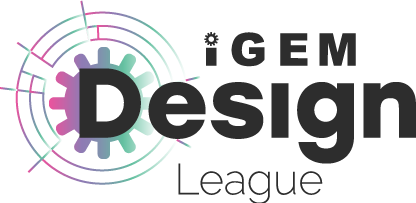
\includegraphics[scale=0.1]{IDL.png}}
\chead{Docking methods}
\usepackage{natbib}
\usepackage{mol2chemfig}
\usepackage{chemfig}

\begin{document}	
	\title {Módulo 8: Actividad 2\\Ciclo de la Urea}
	\date{28 Noviembre 2021}
	\author{Gerardo Cendejas Mendoza\\ Facultad de Ciencias UNAM\\BMC II}
	
	\maketitle
	
	El ciclo de la Urea y el ciclo de Krebs están interrelacionados mediante un sistema llamado ``lanzadera Aspartato--Malato". Esta lanzadera se llama así debido a los dos intermediarios aspartato y malato, son transportados desde el interior y hacia el exterior de la mitocondria, respectivamente. Ninguno de éstos dos intermediarios pertenecen ni a Krebs ni a Urea. Explica ¿cómo es que se relacionan el ciclo de Krebs y el de la Urea a través de éstos intermediarios?
	
	\FloatBarrier
	\begin{figure}[h]
		\centering
		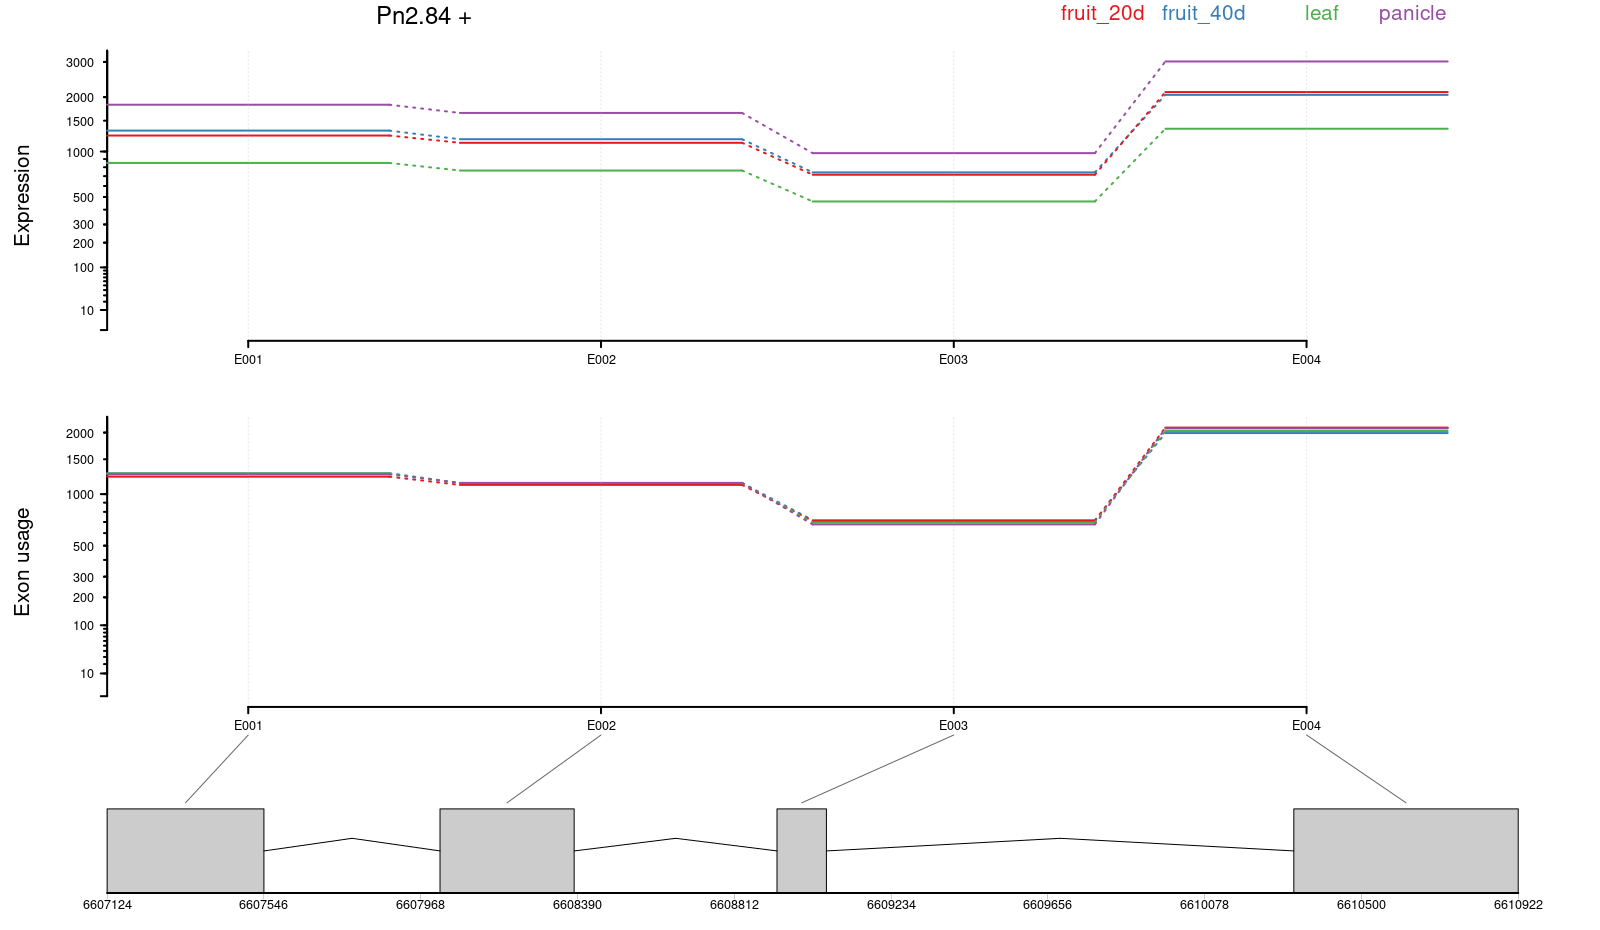
\includegraphics[scale=0.3]{../2/Transcripts/6.png}
		\caption{Algo}
	\end{figure}
	\FloatBarrier
	
	\newpage
	
	El ciclo de Krebs y el ciclo de la urea se relacionan porque en la mitocondria y en el citoplasma se encuentran isoenzimas que llevan a cabo las mismaas reacciones, de convertir fumarato a malato, este a oxalacetato y este a aspartato. Además, como resultado del ciclo de la urea se obtiene fumarato, que es un intermediario del ciclo de Krebs y mediante la lanzadera de Apartato--Malato puede entrar a la matriz mitocondrial y entrar al ciclo de Krebs. De igual manera, a partir del oxalacetato del ciclo de Krebs se puede generar Aspartato, el cual por la misma lanzadera puede salir de la mitocondria y llegar al citosol, aquí puede entrar al ciclo de la urea, pues es necesario en este para la obtención de arginosuccinato a partir de citrulina.
	\newline
	
	\chemfig{O=[:90](-[:30,,,1]OH)-[:150](-[:90,,,1]NH_2)-[:210]-[:150]-[:90]%
-[:150]-[:210](-[:330,,,,draw=none]\mcfcringle{1.3})-[:270]-[:330](-[:30])}

	
\end{document}